% This file was created by tikzplotlib v0.9.1.
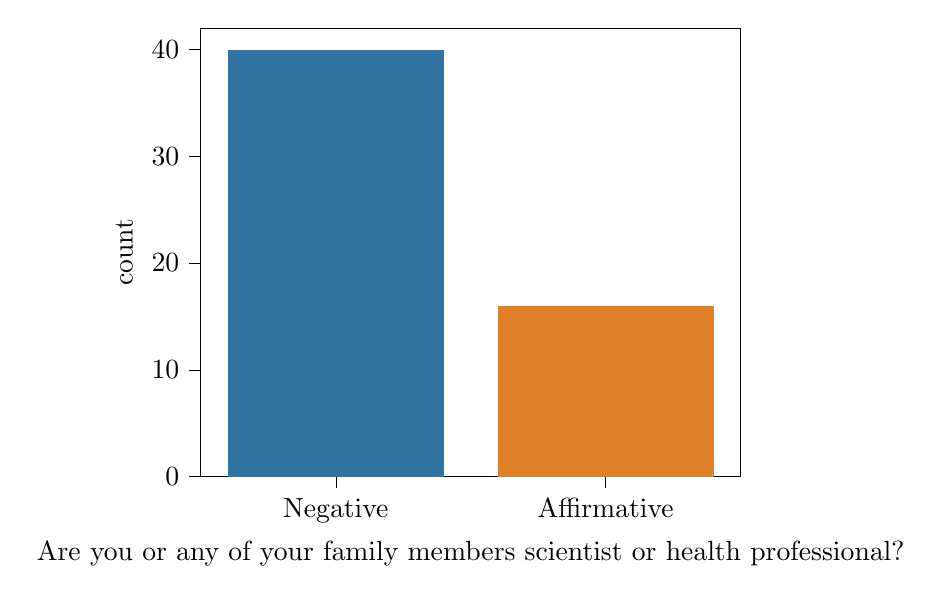
\begin{tikzpicture}

\definecolor{color0}{rgb}{0.194607843137255,0.453431372549019,0.632843137254902}
\definecolor{color1}{rgb}{0.881862745098039,0.505392156862745,0.173039215686275}

\begin{axis}[
tick align=outside,
tick pos=left,
x grid style={white!69.0196078431373!black},
xlabel={Are you or any of your family members scientist or health professional?},
xmin=-0.5, xmax=1.5,
xtick style={color=black},
xtick={0,1},
xticklabels={Negative,Affirmative},
y grid style={white!69.0196078431373!black},
ylabel={count},
ymin=0, ymax=42,
ytick style={color=black}
]
\draw[draw=none,fill=color0] (axis cs:-0.4,0) rectangle (axis cs:0.4,40);
\draw[draw=none,fill=color1] (axis cs:0.6,0) rectangle (axis cs:1.4,16);
\end{axis}

\end{tikzpicture}
